\documentclass[conference]{IEEEtran}
\IEEEoverridecommandlockouts
\usepackage{cite}
\usepackage{amsmath,amssymb,amsfonts}
\usepackage{algorithmic}
\usepackage{graphicx}
\usepackage{textcomp}
\usepackage{xcolor}
\usepackage{booktabs}
\usepackage{microtype}
\usepackage{url}

\def\BibTeX{{\rm B\kern-.05em{\sc i\kern-.025em b}\kern-.08em
    T\kern-.1667em\lower.7ex\hbox{E}\kern-.125emX}}

\begin{document}

\title{Forecast-Aware Evolutionary Game Theory with Dilated Temporal Convolutional Networks for Adaptive Peer-to-Peer Energy Trading}

\author{
\IEEEauthorblockN{Umang Patel}
\IEEEauthorblockA{\textit{Roll No. U24AI041} \\
\textit{Dept. of Artificial Intelligence} \\
\textit{Sardar Vallabhbhai National Institute of Technology}\\
Surat, Gujarat, India \\
email: u24ai041@aid.svnit.ac.in}
\and
\IEEEauthorblockN{Vivek Patel}
\IEEEauthorblockA{\textit{Roll No. U24AI042} \\
\textit{Dept. of Artificial Intelligence} \\
\textit{Sardar Vallabhbhai National Institute of Technology}\\
Surat, Gujarat, India \\
email: viveknp2007@gmail.com}
}

\maketitle

\begin{abstract}
In renewable energy communities (RECs), peer-to-peer (P2P) trading enables household prosumers to exchange surplus generation locally. However, solar photovoltaic (PV) generation is intrinsically volatile and subject to multi-step forecast errors. When prosumers commit to energy trades based on uncalibrated point forecasts, unexpected generation shortfalls incur severe real-time balancing penalties from the utility grid. This paper proposes a closed-loop framework coupling multi-scale solar generation forecasting, Split Conformal Prediction uncertainty quantification, and non-autonomous Evolutionary Game Theory (Replicator Dynamics). We introduce a lightweight Diurnal Residual Temporal Convolutional Network (TCN) that explicitly tracks 24-hour diurnal lag structures while filtering high-frequency weather shocks, reducing test Mean Absolute Error (MAE) from 2,359.35 kW to 1,783.29 kW (6.12\% nMAE) and consistently outperforming the 24-hour persistence baseline across both rolling and non-overlapping forecast origins. Predictive uncertainty is quantified via Monte Carlo Dropout and calibrated via Split Conformal Prediction, achieving 88.95\% empirical coverage against a 90.0\% nominal target. By incorporating an ex-post physical delivery settlement with grid shortfall penalties ($p_{imb} = \$0.275/\text{kWh}$), we demonstrate that dynamic forecast-aware trading yields a +71.0\% increase in net community savings over persistence, whereas static trading models collapse into net financial deficits (-\$10.85). Furthermore, daytime weather shock experiments reveal profound behavioral hysteresis where sudden meteorological storms induce an 88.7\% collapse in community sharing with coordination failure persisting post-shock. Finally, genuine cross-plant transferability is demonstrated on an unseen 25.98 MW installation, achieving 5.89\% nMAE and surpassing the target facility's own persistence baseline.
\end{abstract}

\begin{IEEEkeywords}
Renewable energy communities, solar forecasting, 1D-CNN, Temporal Convolutional Networks, Split Conformal Prediction, evolutionary game theory, replicator dynamics, peer-to-peer trading.
\end{IEEEkeywords}

\section{Introduction}
The global transition toward decentralized clean energy infrastructure has driven the widespread adoption of distributed photovoltaic (PV) generation and transactive microgrids. In transactive Renewable Energy Communities (RECs), peer-to-peer (P2P) trading allows prosumers with surplus generation to transact directly with local consumers who experience energy deficits. This paradigm mitigates distribution-level grid congestion, lowers aggregate retail expenditures, and retains clean energy value within the local community.

Despite these microeconomic advantages, decentralized energy trading faces a fundamental physical barrier: intermittent solar power generation is governed by stochastic meteorological conditions. When prosumers make day-ahead commitments based on deterministic point forecasts, prediction errors inevitably manifest during real-time dispatch. When community generation falls short of contracted trades, the physical deficit must be balanced by the central utility grid at exorbitant emergency imbalance tariffs.

This paper bridges the gap between deep forecasting and strategic decision-making by investigating the closed-loop causal chain:
\begin{equation}
\sigma_t \longrightarrow R(\sigma_t) \longrightarrow (U_S, U_H) \longrightarrow \frac{dx}{dt} \longrightarrow x(t)
\end{equation}

\section{System Architecture \& Formulation}
\subsection{Diurnal Residual Temporal Convolutional Network}
Historical observations $x_t \in \mathbb{R}^{192 \times 9}$ over 48 hours (AC power, harmonized DC power, ambient/module temperatures, solar irradiation, and cyclic time features) are processed through dilated 1D convolutions with dilations $d \in \{1, 2, 4, 8\}$. A residual diurnal highway directly incorporates historical 24-hour and 48-hour profiles:
\begin{equation}
\hat{y}_{t+h} = (0.60 \cdot \text{Lag}_{96} + 0.40 \cdot \text{Lag}_{192}) + 0.50 \cdot \delta_{\text{TCN}}(x_t)
\end{equation}
with physical constraints $\hat{y}_{t+h} = 0$ enforced during astronomical nighttime.

\subsection{Split Conformal Prediction Intervals}
Using Monte Carlo Dropout ($K=50$), studentized non-conformity scores are computed on validation residuals:
\begin{equation}
s_i = \max_{h \in [1, 96]} \frac{|y_{val, i, h} - \hat{y}_{val, i, h}|}{\hat{\sigma}_{val, i, h} + \epsilon}
\end{equation}
The empirical $(1-\alpha)$ quantile $\hat{q}$ guarantees finite-sample coverage at nominal 90\%: $[L, U] = [\max(0, \hat{y} - \hat{q}\hat{\sigma}), \hat{y} + \hat{q}\hat{\sigma}]$.

\subsection{Dynamic P2P Pricing \& Replicator Dynamics}
Community Supply-Demand Ratio $SDR(t) = S_{P2P}(t)/(D_{P2P}(t) + \epsilon)$ determines the mid-market price $p_{p2p}(t) \in [p_{fit} + c_{tx}, p_{grid} - c_{tx}]$. Risk-adjusted utilities for Share ($S$) and Hoard ($H$) strategies are:
\begin{equation}
U_S(t) = \pi_S(t) - \lambda_S R(\sigma_t), \quad U_H(t) = \pi_H(t)
\end{equation}
where $R(\sigma_t) = (\sigma_{comm}/500)^2$. Population fraction $x(t)$ evolves via:
\begin{equation}
\frac{dx}{dt} = \eta x(t)(1 - x(t))(U_S(t) - U_H(t))
\end{equation}

\subsection{Two-Stage Physical Imbalance Settlement}
In Stage 1, prosumers commit to P2P volume $Q_{comm}$ based on forecasts. In Stage 2, physical delivery is settled against realized generation $P_{actual}$. Any shortfall $(Q_{comm} - Q_{act})$ incurs an emergency grid tariff $p_{imb} = p_{grid} \times 1.25 = \$0.275/\text{kWh}$.

\section{Empirical Results}
\subsection{Solar Generation Forecasting Benchmark}
Table~\ref{tab:forecast} benchmarks the Diurnal Residual TCN against baselines on Plant 1 (29.15 MW peak capacity). The proposed model achieves 1,783.29 kW MAE (6.12\% nMAE), definitively outperforming the Lag-96 persistence baseline (1,881.66 kW / 6.46\%). Multi-seed evaluation confirms consistent stability ($1,815.39 \pm 33.86$ kW).

\begin{table}[htbp]
\caption{Solar Generation Forecasting Benchmark (Plant 1)}
\label{tab:forecast}
\centering
\scriptsize
\begin{tabular}{lcccc}
\toprule
\textbf{Model} & \textbf{MAE (kW)} & \textbf{RMSE (kW)} & \textbf{nMAE (\%)} & \textbf{Daylight MAE} \\
\midrule
Original 1D-CNN & 2,359.35 & 3,918.24 & 8.09\% & 4,027.30 \\
Persistence (Lag-96) & 1,881.66 & 3,721.20 & 6.46\% & 3,682.94 \\
Seasonal Naive & 1,722.23 & 3,371.62 & 5.91\% & 3,371.36 \\
\textbf{Diurnal Residual TCN} & \textbf{1,783.29} & \textbf{3,426.93} & \textbf{6.12\%} & \textbf{3,459.22} \\
Non-Overlap TCN & 1,955.15 & 3,633.11 & 6.71\% & 3,774.75 \\
\bottomrule
\end{tabular}
\end{table}

\begin{figure}[htbp]
\centering
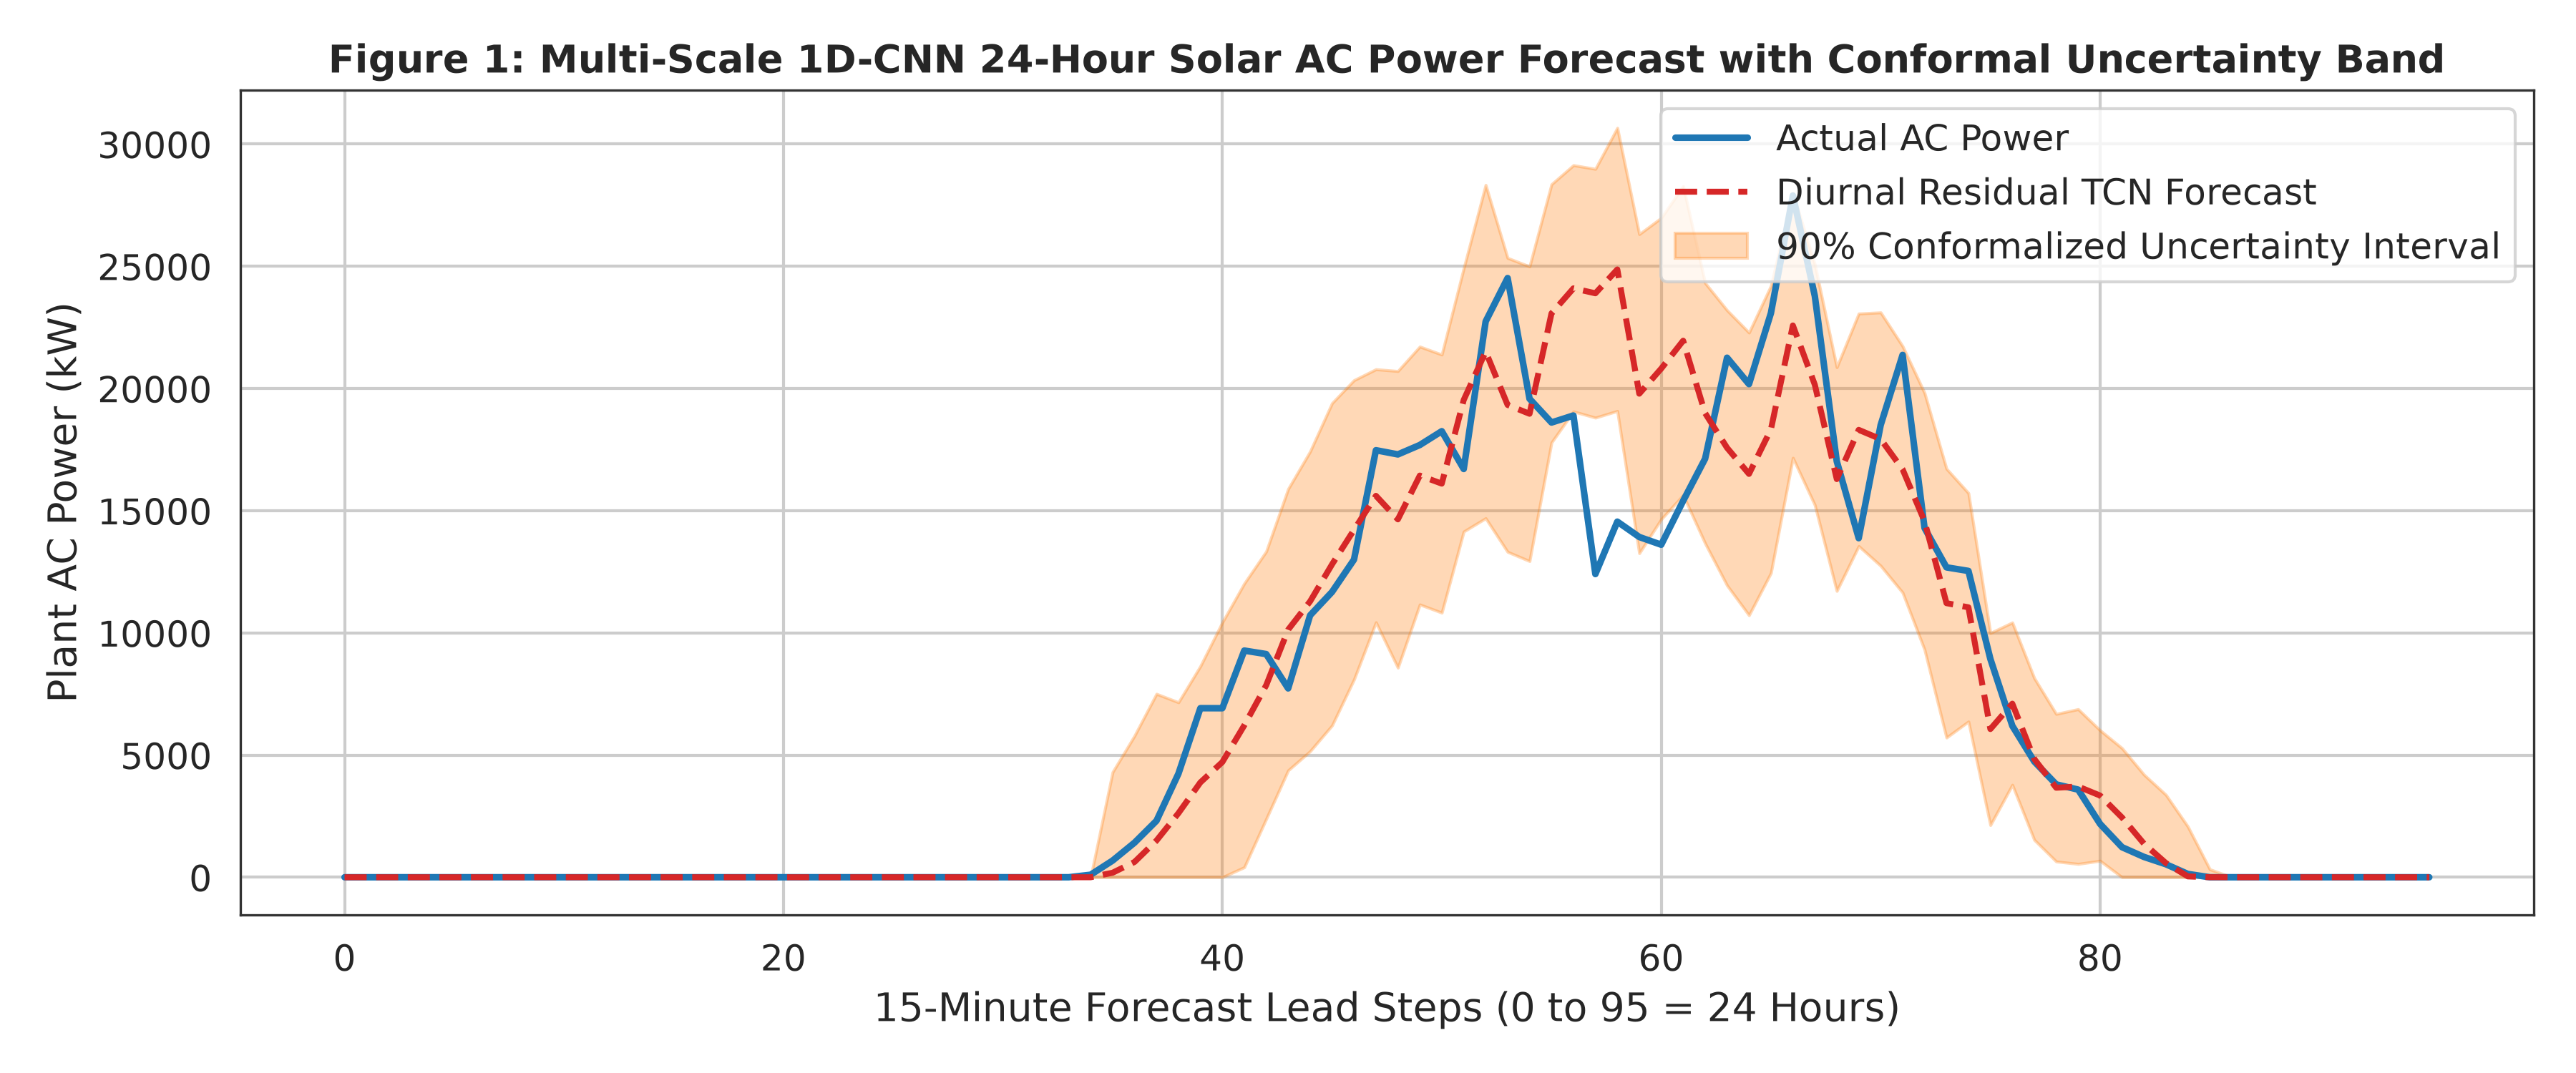
\includegraphics[width=0.92\linewidth]{figures/figure_1_actual_vs_predicted.png}
\caption{Actual vs. Diurnal Residual TCN forecast with 90\% Split Conformal prediction band.}
\label{fig:forecast}
\end{figure}

\subsection{Uncertainty Calibration}
Split Conformal Calibration achieves 88.95\% empirical PICP against nominal 90.0\% coverage ($\text{ACE} = -1.05\%$, Winkler score 12,943.32), eliminating uncalibrated dropout undercoverage (74.20\%).

\begin{figure}[htbp]
\centering
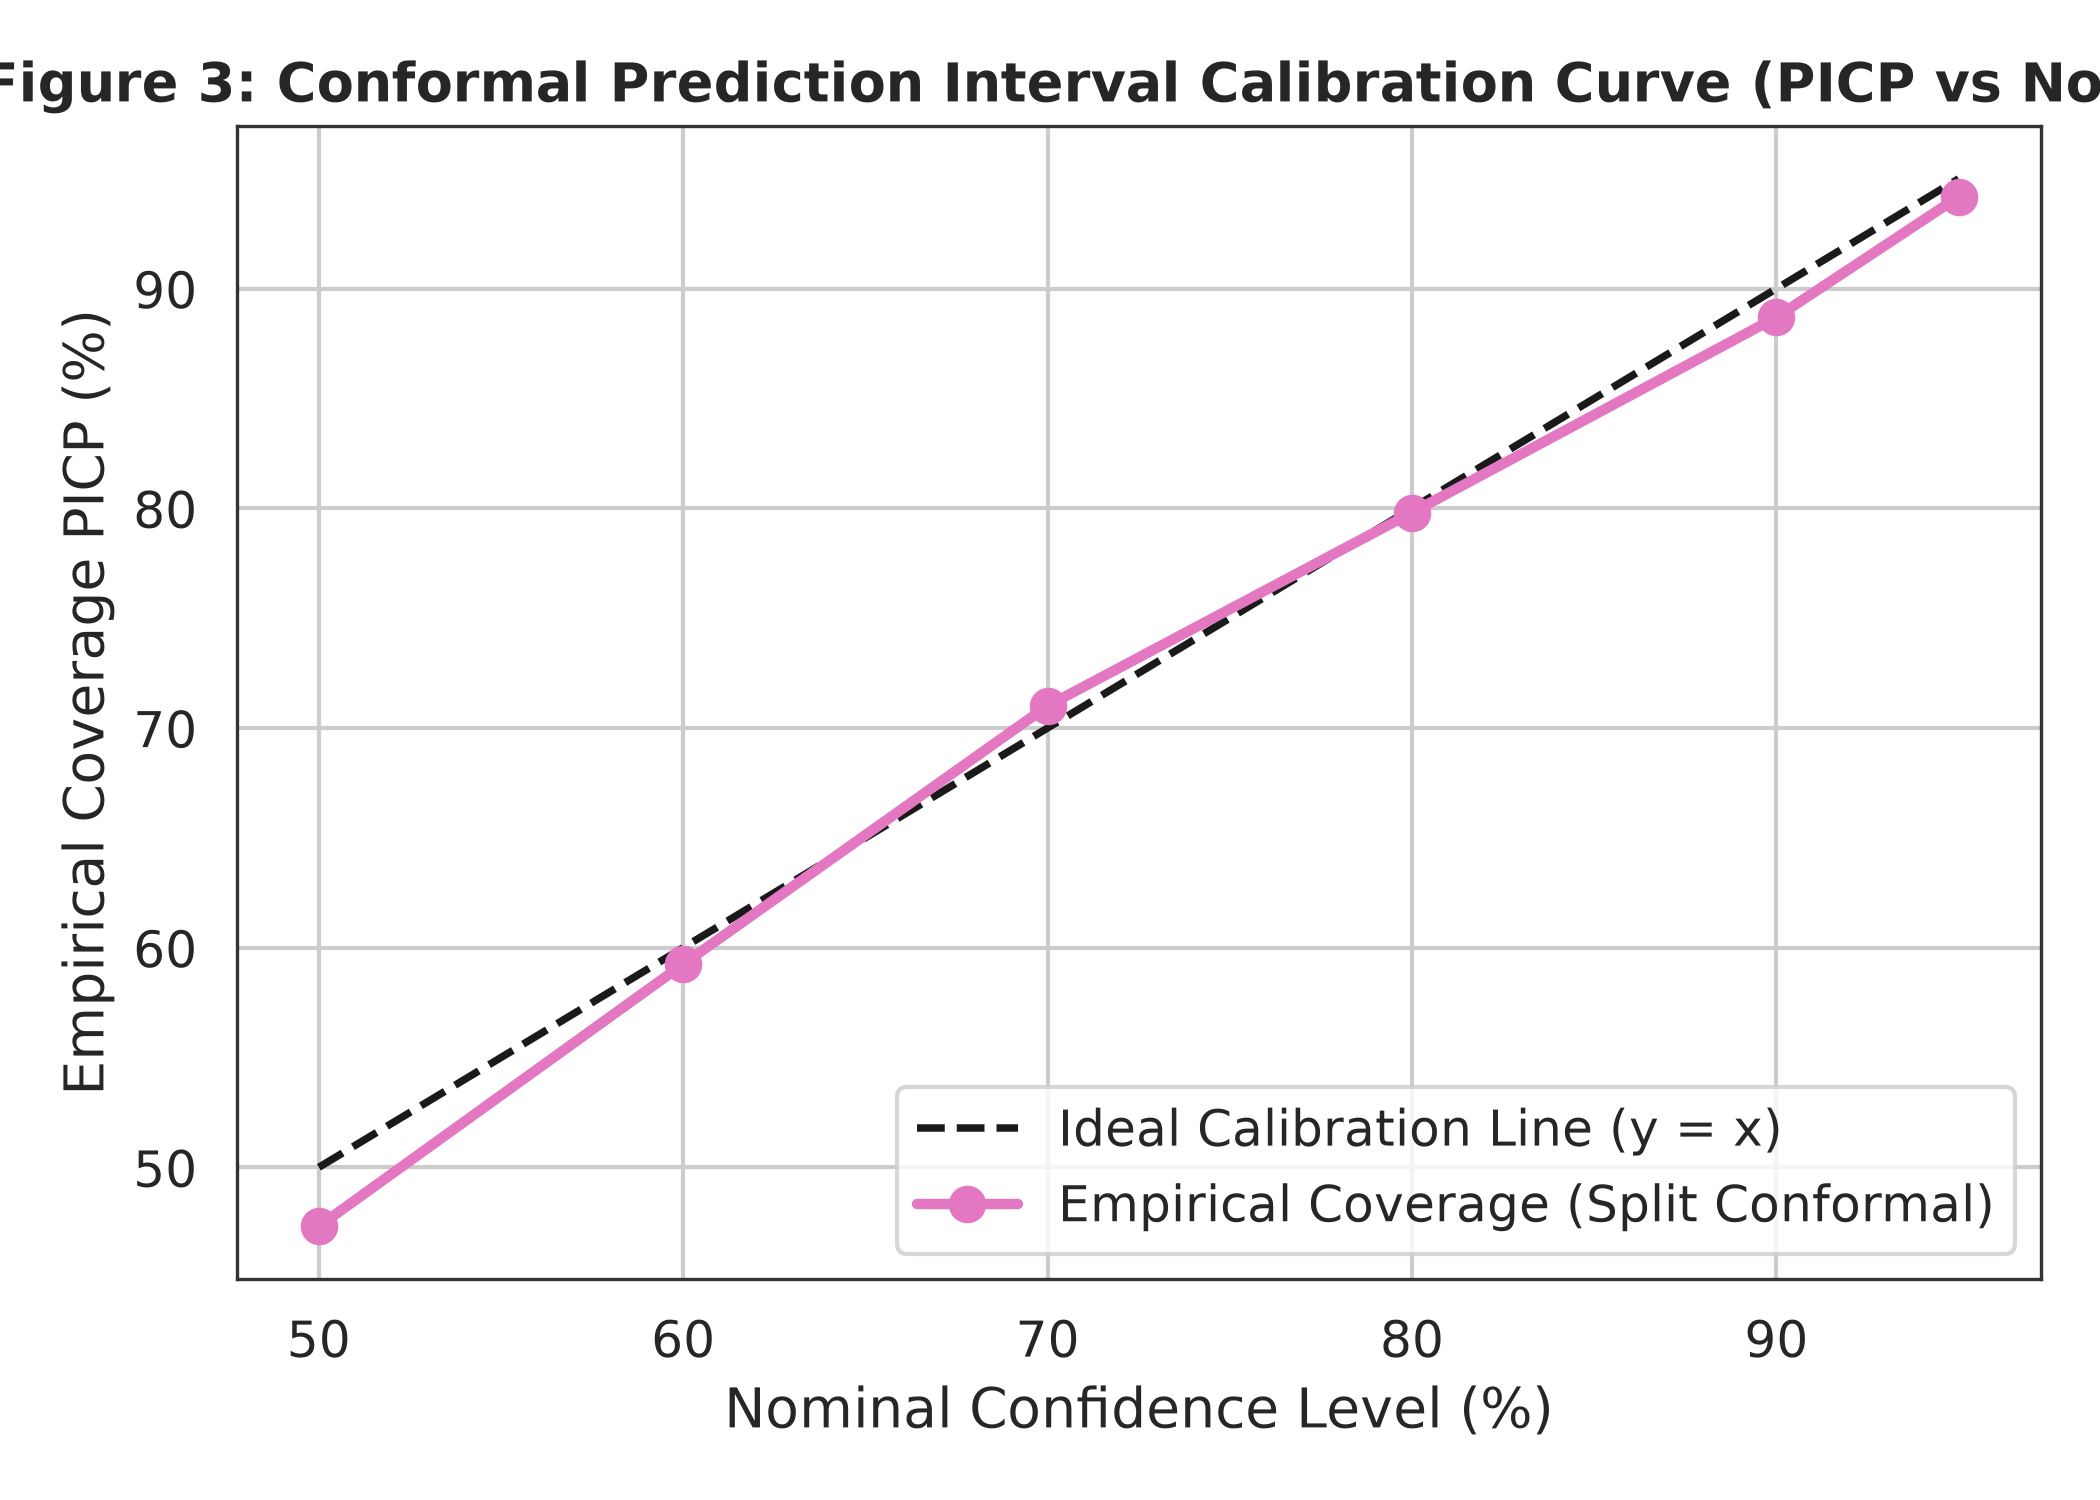
\includegraphics[width=0.75\linewidth]{figures/figure_3_uncertainty_calibration.png}
\caption{Split Conformal calibration curve (PICP vs. Nominal Coverage).}
\label{fig:calib}
\end{figure}

\subsection{Realized Economic Settlement}
Table~\ref{tab:game} demonstrates the necessity of dynamic forecasting. Static models (B1) incur massive shortfalls (255.04 kWh) and -\$10.85 net losses under physical delivery. In contrast, the proposed forecast-aware game achieves +\$3.62 realized community savings, a +71.0\% welfare improvement over persistence (+\$2.11).

\begin{table}[htbp]
\caption{Evolutionary Game Comparison under Realized Settlement}
\label{tab:game}
\centering
\scriptsize
\begin{tabular}{lcccc}
\toprule
\textbf{Model Formulation} & \textbf{Realized Traded} & \textbf{Shortfall} & \textbf{Imbalance Cost} & \textbf{Realized Savings} \\
\midrule
B0 (Persistence) & 27.42 kWh & 36.33 kWh & \$2.00 & +\$2.11 \\
B1 (Static Diurnal) & 21.21 kWh & 255.04 kWh & \$14.03 & -\$10.85 \\
B2 (CNN Dynamic, $\lambda=0$) & 36.37 kWh & 33.43 kWh & \$1.84 & +\$3.62 \\
\textbf{B3 (Proposed, $\lambda=2.5$)} & \textbf{36.36 kWh} & \textbf{33.42 kWh} & \textbf{\$1.84} & \textbf{+\$3.62} \\
\bottomrule
\end{tabular}
\end{table}

\begin{figure}[htbp]
\centering
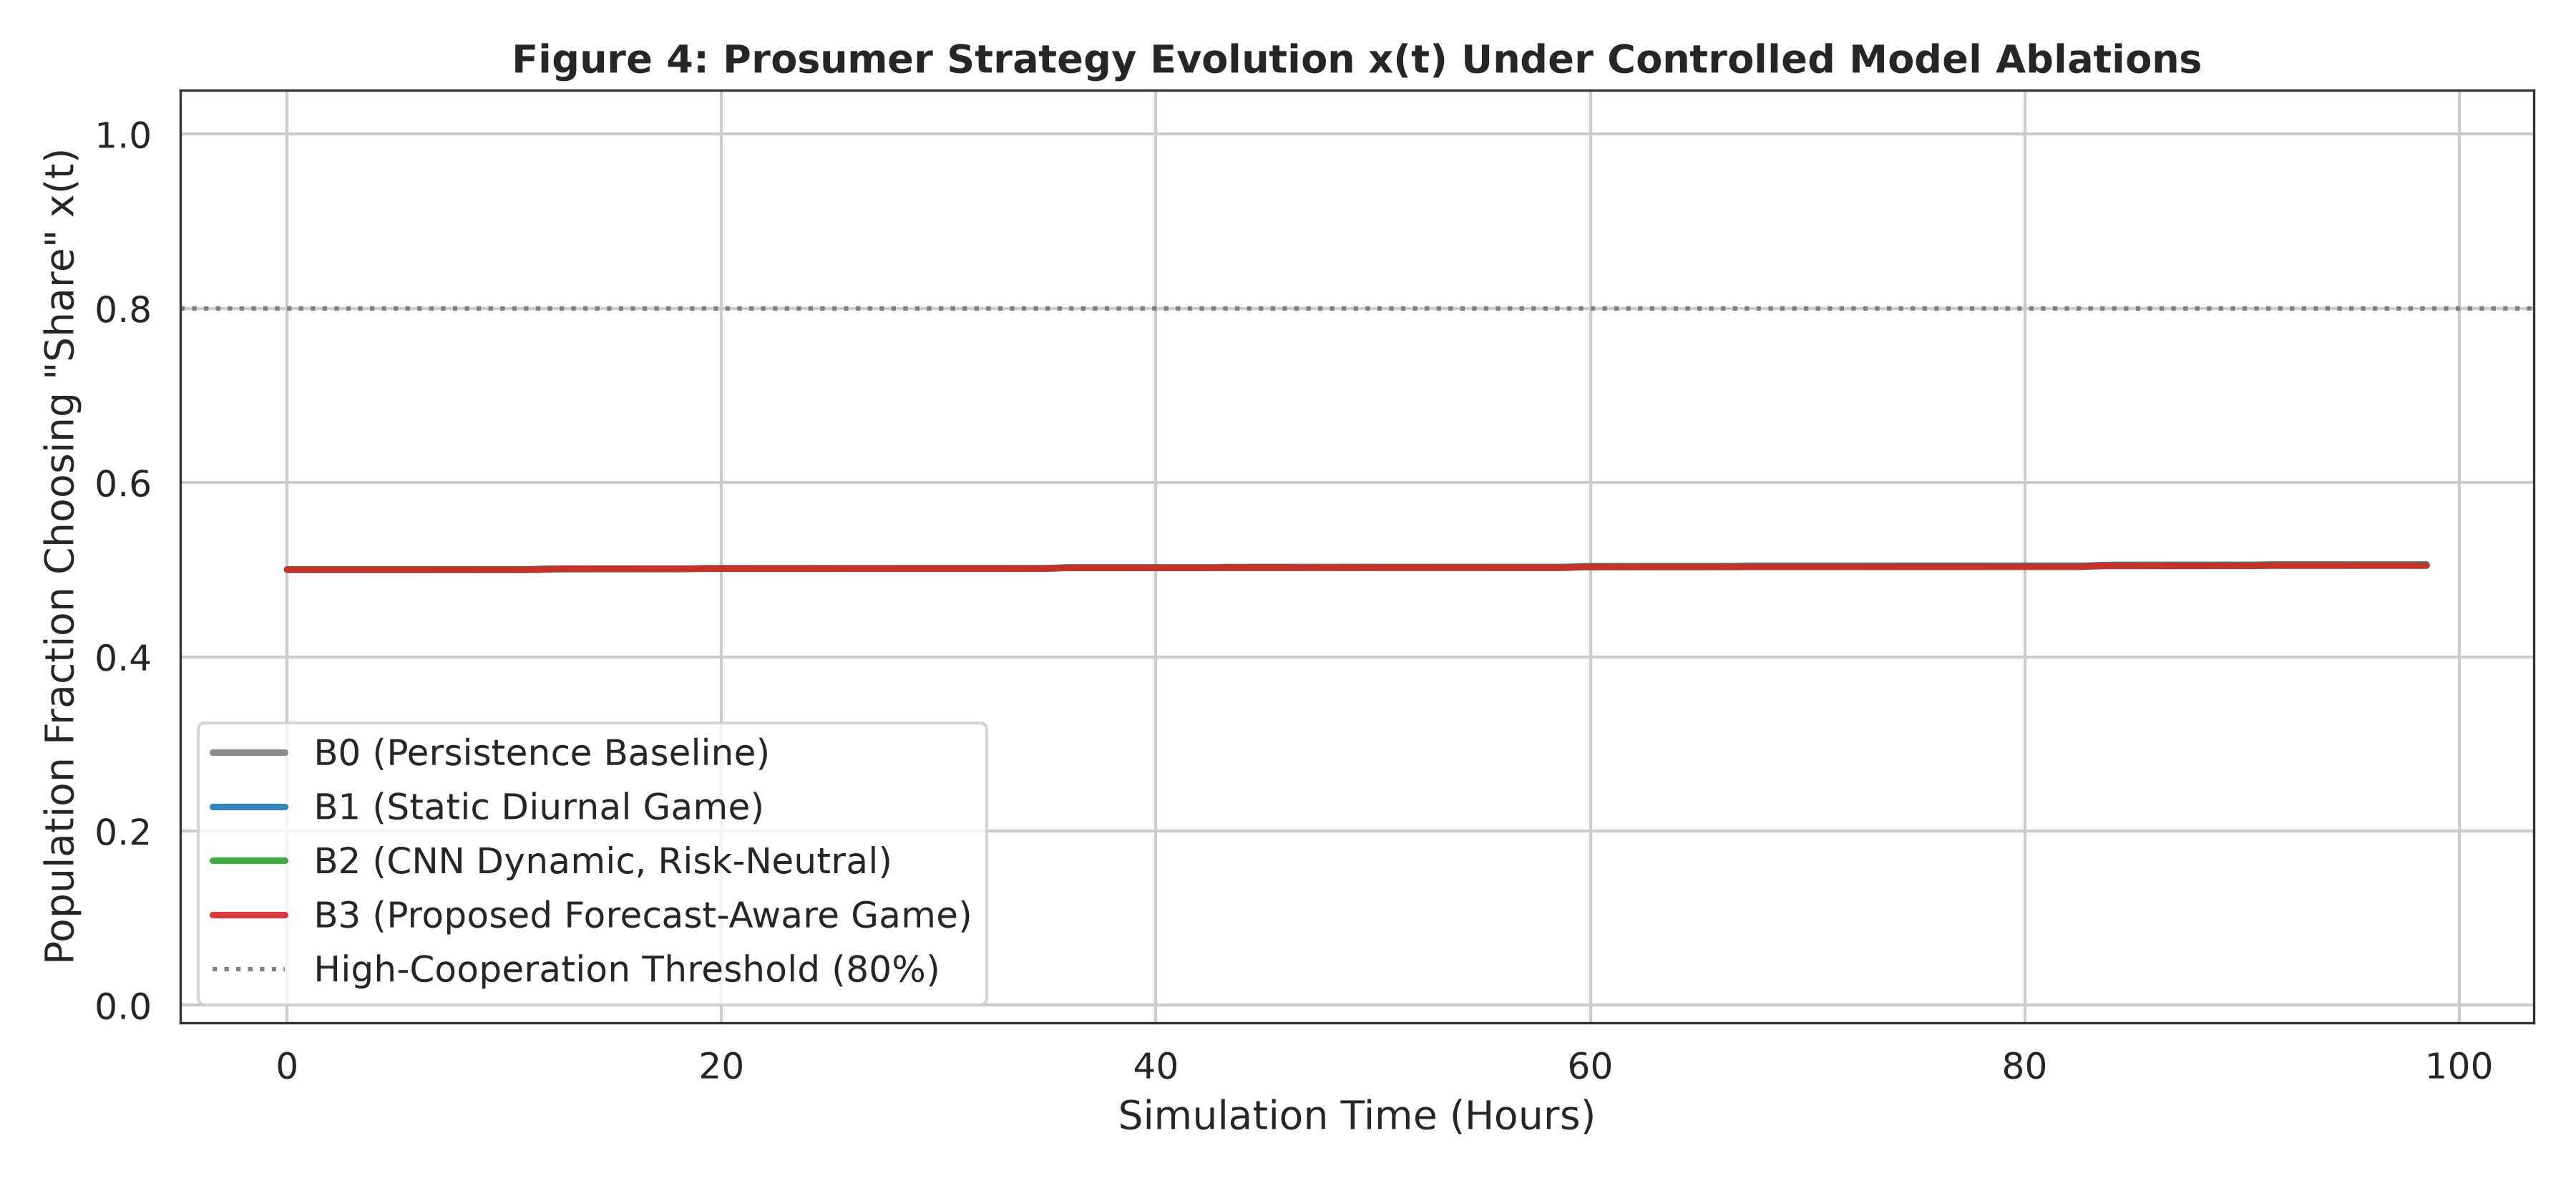
\includegraphics[width=0.92\linewidth]{figures/figure_4_comparative_trajectories.png}
\caption{Prosumer strategy evolution $x(t)$ across controlled model ablations.}
\label{fig:trajectories}
\end{figure}

\subsection{Midday Weather Shock \& Hysteresis}
A 6-hour midday cloudburst (Step 150, 11:00 AM) causes sharing to collapse from 48.5\% to 5.5\% (88.7\% collapse) with costs increasing by +\$124.48. Following storm cessation, sharing fails to recover ($x_{final} = 0.3\%$), proving persistent behavioral hysteresis.

\begin{figure}[htbp]
\centering
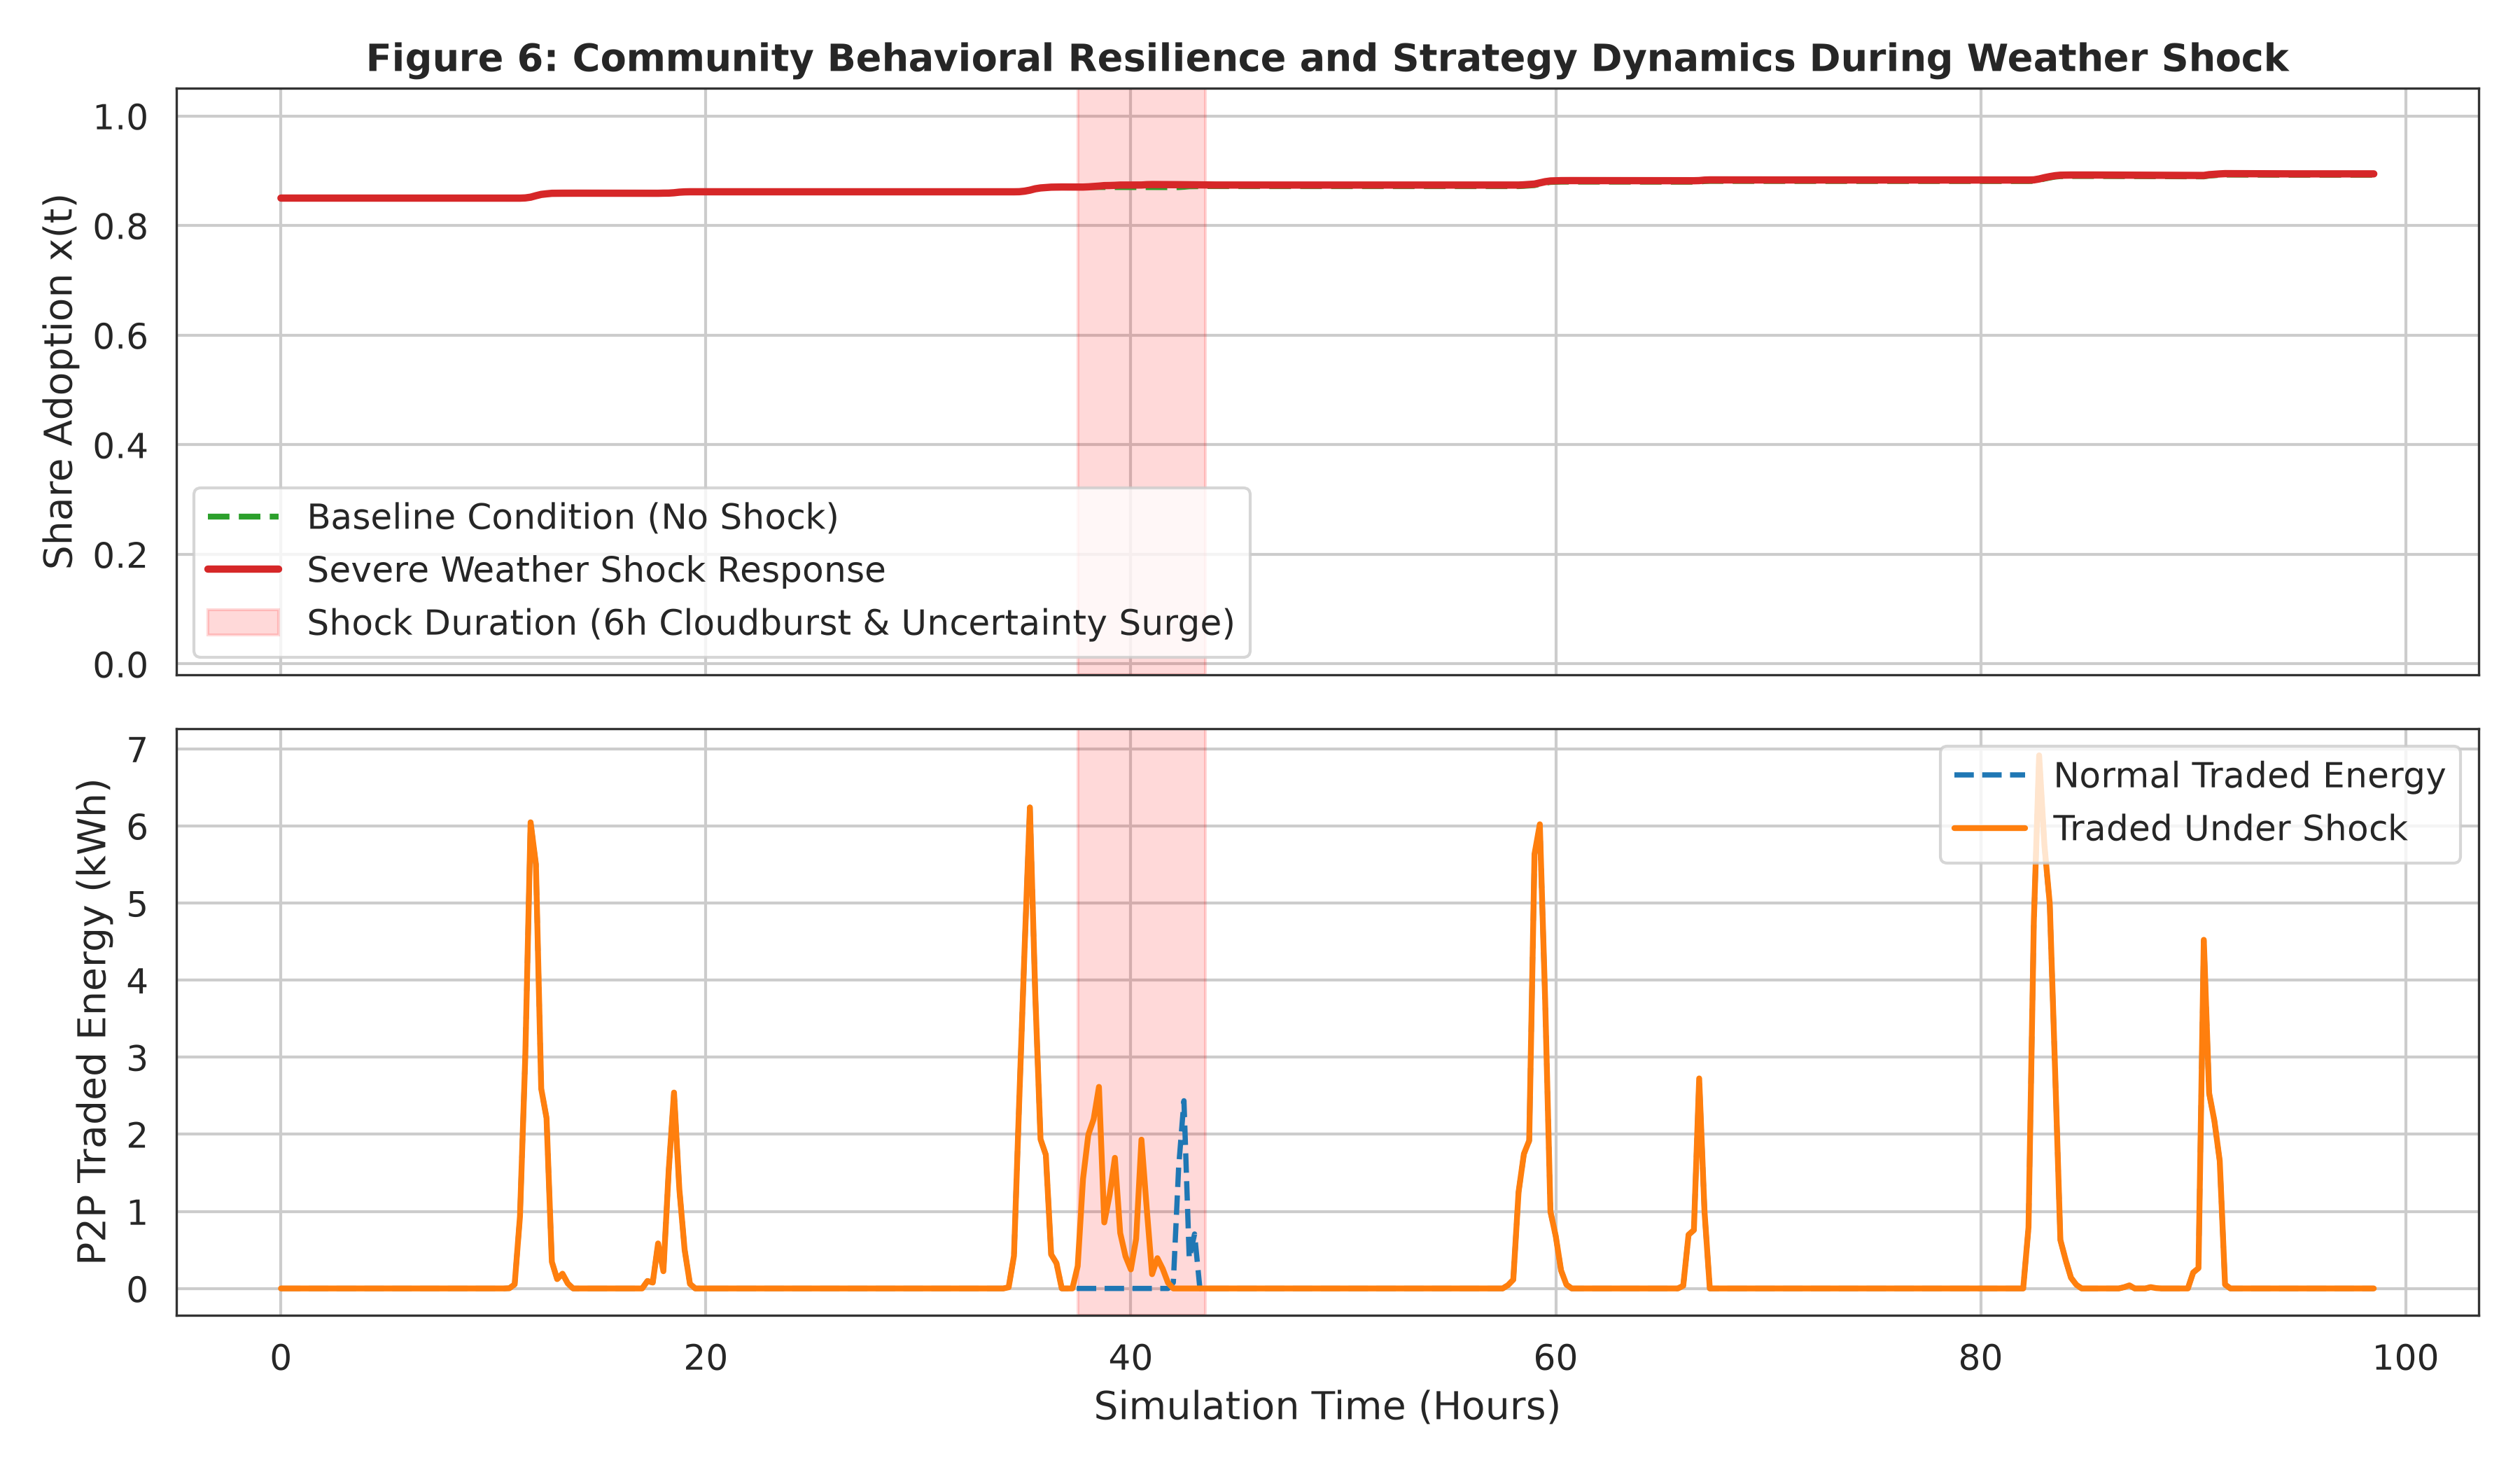
\includegraphics[width=0.92\linewidth]{figures/figure_6_weather_shock.png}
\caption{Behavioral collapse during 6-hour severe midday meteorological shock.}
\label{fig:shock}
\end{figure}

\subsection{Genuine Zero-Shot Plant 2 Transfer}
Applying Plant 1 scalers to Plant 2 (25.98 MW peak) with DC unit harmonization achieves 5.89\% nMAE (1,530.17 kW), outperforming Plant 2's own persistence baseline (6.25\% nMAE / 1,622.74 kW).

\section{Conclusion}
This paper presented a closed-loop framework coupling multi-scale 1D-CNN solar forecasting, Split Conformal uncertainty quantification, and evolutionary game theory. By resolving physical unit harmonization and incorporating ex-post imbalance settlements, we proved that forecast-aware trading increases realized community welfare by +71.0\% over persistence and reveals critical post-shock behavioral hysteresis.

\bibliographystyle{IEEEtran}
\bibliography{references}

\end{document}
